\section{System Design (Saroj)}
\label{sec:system_design}
\begin{itemize}
    \item KWS design
    \item Figure
\end{itemize}

%%% FIGURE: KWS ARCHITECTURE
%%% ------------------------
\begin{figure}[htbp]	
    %\centerline{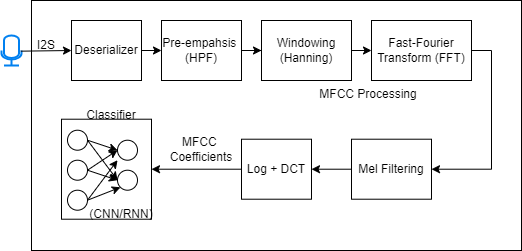
\includegraphics{figs/KWS-architecture.png}}
    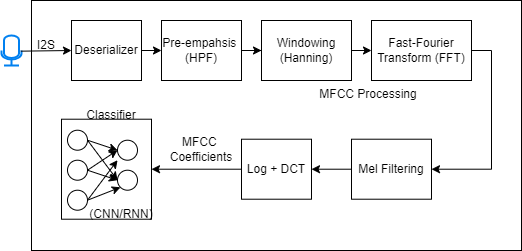
\includegraphics[width=0.45\textwidth]{figs/KWS-architecture.png}
    \caption{Implementation of a Keyword Spotter (KWS) [\textbf{FIXME}: Move the CNN to the host processor]}
    \label{fig:KWS_Arch}
\end{figure}

Acoustic audio analysis is widely used for important applications including heart monitoring, keyword spotting (KWS), and the preventative maintenance of heavy machinery \cite{chong20220}. 
Among these methods, keyword spotting (KWS) plays a crucial role in various voice-activated smart assistants like Google Assistant and Amazon Alexa.
Figure~\ref{fig:KWS_Arch} illustrates a well-known design of a digital KWS architecture \cite{chong20220}. This design employs Mel frequency cepstral coefficients (MFCC) to derive spectral audio features from the input audio signal.
In this configuration, a digital microphone collects live data via an $I^2S$ serial interface. This stream of data is then converted to parallel bytes. The low-frequency portion of the signal is eliminated by applying a pre-emphasis filter (high-pass filter or HPF). The pre-emphasis filter is commonly realized by the following difference equation:
%%Equation: HPF
\begin{equation}
    y[n] = x[n] - \alpha~x[n-1] \label{eq:hpf}
\end{equation}
where, $\alpha$ is typically in the $0.9-1$ range \cite{han2006efficient}.  
After the pre-emphasis filter is applied, the data is subjected to a window function (e.g., Hamming, Hanning, etc.) to prevent spectral leakage during the FFT operation.
After applying the window function, a fast fourier transform (FFT) is performed on the signal to identify its frequency components. The linear frequency scale obtained from the FFT is known to be inadequate for replicating how the human ear perceives sound. Thus, the linear frequency spectrum is transformed into the Mel logarithmic scale, as given by \cite{han2006efficient}:
%% Equation: Mel-log filter
\begin{equation}
    Mel(f) = 2595\cdot \log_{10}\left({1 + \frac{f}{700}}\right) \label{eq:mel-log}
\end{equation}
After applying the Mel log filter, the logarithm of the Mel frequency power is calculated, followed by a Discrete Cosine Transform (DCT) to derive the MFCC coefficients. These MFCC coefficients are then utilized to classify the voice signal using a classifier such as a convolutional neural network (CNN), recurrent neural network (RNN), long short term memory (LSTM), or other similar techniques \cite{mahmood2021speech}.

Despite the architecture's popularity for KWS, the hardware implementation can differ greatly based on the application, which involves various trade-offs between power, area, and accuracy.
For this research, a \textit{smart microphone } application was examined in which the KWS is embedded directly into the microphone. This configuration allows it to recognize one or more keywords with moderate accuracy, while consuming minimum power while occupying a small area.
Now, each component is reviewed and determined on how to refine the design for this application. Digital microphones are generally built to record audio frequencies up to 22~kHz with a sample precision ranging from 12-16 bits. After capturing a keyword sample such as "Wakeup Neo", the data underwent low-pass filtering and reduction in precision using an open-source audio tool \textit{Audacity}. This procedure was progressively repeated until a noticeable effect was observed. Following multiple iterations, a 4 kHz bandwidth and 7-bit fixed-point precision were deemed adequate for the operation, resulting in significant area and power savings at the cost of minimal accuracy.
A similar optimization was performed for the HPF (Eq.~\ref{eq:hpf}) by selecting $\alpha=31/32=0.969$, which can be implemented using a basic \textit{shift-and-add} operation rather than a hardware multiplier. 
A hanning window was selected for the windowing function, and the coefficients were implemented using exclusively single shift operations, resulting in substantial hardware savings with a minor increase in spectral leakage. 
Besides CNN, FFT is the next largest hardware component with respect to area and power consumption. The $Radix-2^2$ single delay feedback ($R2^2SDF$) is a design that is efficient in both area and power usage, given that it utilizes the fewest multipliers and adders compared to other FFT hardware implementations. An optimization using \textit{spectrogram} was employed to determine a 32-point FFT that results in lower frequency bins with the benefit of significant hardware savings.
Equivalent hardware reductions were achieved by employing rectangular Mel filter bins as opposed to triangular ones, with only a slight reduction in accuracy. 
Lastly, the DCT calculation is reduced, which compromises some accuracy. The host then utilizes these MFCC coefficients with classifiers such as CNN or RNN to spot the trained keyword.

[\textbf{FIXME} Need to decide if we want to mention agentic flow for architectural phase]

%%% ------------------------
%%% Agentic-AI Generative HW
%%% ------------------------
\subsection{Agentic-AI Generative Hardware}

Once the architecture is finalized, the components are described using a hardware description language such as Verilog and the design undergoes verification. 

[\textbf{FIXME} Discuss and write this section...]

After verification, the hardware model is transformed into a manufacturable layout using a series of tools outlined in the following section.

%%% ------------------------
%%% RTL-to-GDS Design Flow
%%% ------------------------
\subsection{RTL-to-GDS Design Flow}

%%% FIGURE: RTL-TO-GDS Desing Flow 
%%% ------------------------
\begin{figure}[htbp]
	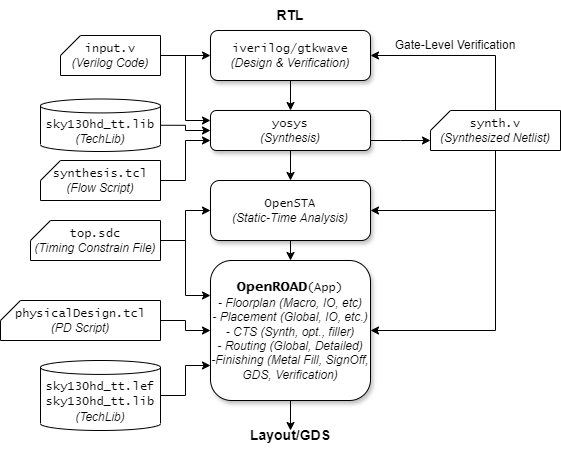
\includegraphics[width=0.45\textwidth]{figs/rtl2gds-toolchain.png}
	\caption{RTL-to-GDS design flow using open-source tools.[\textbf{FIXME}: Add detail to the OpenROAD flow]}
	\label{fig:RTL-to-GDS}
\end{figure}

After the design has been verified and finalized, physical design tools are employed to transform the abstract hardware model into its physical form (GDSII). Figure~\ref{fig:RTL-to-GDS} illustrates a physical design flow utilizing a chain of open-source tools. The first step in the physical design (PD) process is \textit{synthesis}, where a tool like \textit{Yosys} synthesizes the Verilog description into a lower-level representation, such as a netlist of logic gates, suitable for physical implementation. In addition to the Verilog design code, Yosys also requires a technology library (\texttt{*.lib}) and a command script (	\texttt{*.tcl}) to perform the synthesis of the Verilog design. Once synthesis is completed, verification usually involves two steps: 1) 	\textit{Formal verification} or gate-level simulation to confirm that the synthesized netlist's functionality aligns with the original Verilog model; 2) Static Timing Analysis (STA) to ensure there are no timing issues across various process corners and temperature conditions. 
The widely adopted tool for Static Timing Analysis (STA) is the open-source software \textit{OpenSTA}. The input to OpenSTA is the synthesized netlist and a timing constrained file (\texttt{*.sdc}). 
After verifying that the timing requirements are met, the physical design is completed using a leading open-source application \textit{OpenROAD} \cite{ajayi2019toward}.
OpenROAD itself contains many complex steps including floorplanning, cell placement, clock-tree synthesis (CTS), routing and finishing steps. In addition, every step involves several substeps, which vary depending on the complexity of the design. Each step utilizes tools and scripts, predominantly written in \textit{Tcl}, to automate the workflow. 

[\textbf{FIXME}: Should we add details of each flow ?]

While OpenROAD aims for "RTL-to-GDS in 24-hours with No-Human-in-Loop (NHIL)", it nevertheless requires a specialist in digital physical design to initiate and manage the flow, and human intervention is still needed to resolve any flow or design issues.
Furthermore, almost every step mentioned calls for \textit{ timing closure}, and an expert usually handles error corrections manually.

[\textbf{FIXME}: Write how agentic flow can integrate into the flow assisted physical design flow for a medium level expert in this field ?]

